\section{Tools}

\subsection{Recommended References}
\begin{frame}{Bayesian Statistics - Recommended References}
	\begin{vfilleditems}
		\item \textcite{geTuringLanguageFlexible2018} - \texttt{Turing.jl} paper
		\item \textcite{carpenterStanProbabilisticProgramming2017} - \texttt{Stan} paper
		\item \textcite{pymc3} - \texttt{PyMC} paper
		\item \href{https://storopoli.github.io/Bayesian-Julia/pages/1_why_Julia/}{Bayesian Statistics with Julia and \texttt{Turing.jl} - Why Julia?}
	\end{vfilleditems}
\end{frame}

\begin{frame}{Tools}
	\centering
	\textit{``A man and his tools make a man and his trade''}

	\vspace{2ex}

	Vita Sackville-West
\end{frame}

\begin{frame}{Tools}
	\begin{vfilleditems}
		\item \LARGE  \href{https://mc-stan.org}{\texttt{Stan}} (BSD-3 License)
		\item \LARGE  \href{https://turing.ml}{\texttt{Turing.jl}} (MIT License)
		\item \href{https://www.pymc.io/}{\texttt{PyMC}} (Apache License)
		\item \small \href{https://mcmc-jags.sourceforge.io/}{\texttt{JAGS}} (GPL License)
		\item \footnotesize \href{https://www.mrc-bsu.cam.ac.uk/software/bugs/}{\texttt{BUGS}} (GPL License)
	\end{vfilleditems}
\end{frame}

\subsection{Stan}
\begin{frame}{\texttt{Stan}\footnote{\textcite{carpenterStanProbabilisticProgramming2017}}}
	\begin{columns}
		\begin{column}{0.8\textwidth}
			\begin{vfilleditems}
				\small
				\item High-performance platform for statistical
				modeling and  statistical computation
				\item Financial support from
				\href{https://numfocus.org/}{NUMFocus}:
				\begin{vfilleditems}
					\footnotesize
					\item AWS Amazon
					\item Bloomberg
					\item Microsoft
					\item IBM
					\item RStudio
					\item Facebook
					\item NVIDIA
					\item Netflix
				\end{vfilleditems}
				\small
				\item Open-source language, similar to \texttt{C++}
				\item Markov Chain Monte Carlo (MCMC) parallel sampler
			\end{vfilleditems}
		\end{column}
		\begin{column}{0.2\textwidth}
			\centering
			
\includegraphics[width=0.9\textwidth]{stan.png}
		\end{column}
	\end{columns}
\end{frame}

\begin{frame}[fragile]{\texttt{Stan} Code Example}
	\begin{lstlisting}[basicstyle=\footnotesize, language=Stan]
        data {
          int<lower=0> N;
          vector[N] x1;
          vector[N] x2;
          vector[N] y;
        }
        parameters {
          real alpha;
          real beta1;
          real beta2;
          real<lower=0> sigma;
        }
        model {
          alpha ~ normal(0, 20);
          beta1 ~ normal(0, 2);
          beta2 ~ normal(0, 2);
          sigma ~ cauchy(0, 2.5);
          y ~ normal(alpha + beta1 * x1 + beta2 * x2, sigma);
        }
    \end{lstlisting}
\end{frame}

\subsection{Turing.jl}
\begin{frame}{\texttt{Turing.jl}\footnote{\textcite{geTuringLanguageFlexible2018}}}
	\begin{columns}
		\begin{column}{0.8\textwidth}
			\begin{vfilleditems}
				\small
				\item Ecosystem of Julia packages for Bayesian
				Inference using probabilistic programming
				\item \href{https://www.julialang.org}{Julia} is a fast
				dynamic-typed language that just-in-time (JIT)
				compiles into native code using LLVM:
				\href{https://www.nature.com/articles/d41586-019-02310-3}{``runs like C but reads like Python''};
				meaning that is \textit{blazing} fast, easy to prototype and read/write code
				\item Julia has Financial support from
				\href{https://numfocus.org/}{NUMFocus}
				\item Composability with other Julia packages
				\item Several other options of Markov Chain Monte Carlo (MCMC) samplers
			\end{vfilleditems}
		\end{column}
		\begin{column}{0.2\textwidth}
			\centering
			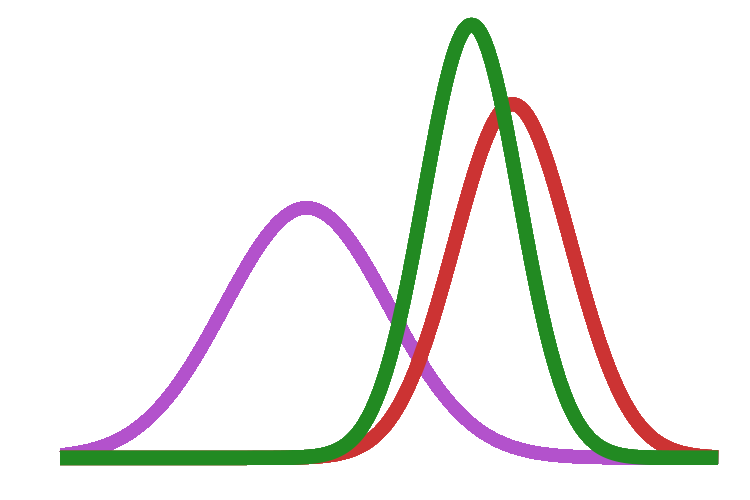
\includegraphics[width=0.9\textwidth]{turing.png}
		\end{column}
	\end{columns}
\end{frame}

\begin{frame}{\texttt{Turing.jl} Ecosystem}
	We have several Julia packages under \texttt{Turing.jl}'s GitHub
	organization \href{https://github.com/TuringLang}{TuringLang},
	but I will focus on 6 of those:

	\begin{vfilleditems}
		\small
		\item \href{https://github.com/TuringLang/Turing.jl}{\texttt{Turing.jl}}:
		main package that we use to \textbf{interface with all
			the Turing ecosystem} of packages and the backbone of
		everything
		\item \href{https://github.com/TuringLang/MCMCChains.jl}{\texttt{MCMCChains.jl}}:
		interface to \textbf{summarizing MCMC simulations} and
		has several utility functions for \textbf{diagnostics}
		and \textbf{visualizations}
		\item \href{https://github.com/TuringLang/DynamicPPL.jl}{\texttt{DynamicPPL.jl}}:
		specifies a domain-specific language for \texttt{Turing.jl},
		entirely written in Julia, and it is modular
		\item \href{https://github.com/TuringLang/AdvancedHMC.jl}{\texttt{AdvancedHMC.jl}}:
		modular and efficient implementation of advanced
		Hamiltonian Monte Carlo (HMC) algorithms
		\item \href{https://github.com/TuringLang/DistributionsAD.jl}{\texttt{DistributionsAD.jl}}:
		defines the necessary functions to enable automatic
		differentiation (AD) of the log PDF functions from
		\href{https://github.com/JuliaStats/Distributions.jl}{\texttt{Distributions.jl}}
		\item \href{https://github.com/TuringLang/Bijectors.jl}{\texttt{Bijectors.jl}}:
		implements a set of functions for transforming constrained
		random variables (\textit{e.g.} simplexes, intervals)
		to Euclidean space
	\end{vfilleditems}
\end{frame}

\begin{frame}[fragile]{\texttt{Turing.jl}\footnote{
			I believe in Julia's potential and wrote a whole set of
			\href{https://storopoli.github.io/Bayesian-Julia}{
				Bayesian Statistics tutorials using Julia and
				\texttt{Turing.jl}} \parencite{storopoli2021bayesianjulia}}
		Code Example}
	\begin{lstlisting}[basicstyle=\small, language=Matlab, escapeinside=\{\}]
        @model linreg({$x_1$}, {$x_2$}, y) = begin
            {$\alpha$} ~ Normal(0, 20)
            {$\beta_1$} ~ Normal(0, 2)
            {$\beta_2$} ~ Normal(0, 2)
            {$\sigma$} ~ truncated(Cauchy(0, 2.5); lower=0)

            y .~ Normal({$\alpha$} .+ {$\beta_1$} * {$x_1$} + {$\beta_2$} * {$x_2$}, {$\sigma$})
        end
    \end{lstlisting}
\end{frame}

\begin{frame}{\texttt{Stan} and \texttt{Julia} mentioned in Billions\footnote{
			If you cannot watch the video \href{https://github.com/storopoli/Bayesian-Statistics/blob/main/images/stan_billions_subtitled.mp4?raw=true}{click here}
			to see it in your browser.} (Season 3 Episode 9)}
	\centering
	\includemedia[
		width=\linewidth,
		height=0.3\linewidth,
		addresource=stan_billions_subtitled.mp4,
		transparent,
		activate=pageopen,
		passcontext,  %show VPlayer's right-click menu
		flashvars={
				source=stan_billions_subtitled.mp4
				&loop=true
				&scaleMode=stretch
			}
	]{\texttt{Stan} and Julia mentioned in Billions}{http://mirrors.ctan.org/macros/latex/contrib/media9/players/VPlayer.swf}
\end{frame}

\subsection{PyMC}
\begin{frame}{\texttt{PyMC}\footnote{\textcite{pymc3}}}
	\begin{columns}
		\begin{column}{0.8\textwidth}
			\begin{vfilleditems}
				\small
				\item Python package for Bayesian statistics
				with a Markov Chain Monte Carlo sampler
				\item Financial support from \href{https://numfocus.org/}{NUMFocus}
				\item Backend was based on \texttt{Theano}
				\item \texttt{Theano} \textbf{died}, but \texttt{PyMC} developers create a fork
				named \texttt{Aesara}
				\item We have no idea what will be the backend in
				the future.
				\texttt{PyMC} developers are still experimenting with other
				backends: \texttt{TensorFlow Probability}, \texttt{NumPyro}
				and so on ...
			\end{vfilleditems}
		\end{column}
		\begin{column}{0.2\textwidth}
			\centering
			
\includegraphics[width=0.9\textwidth]{pymc.png}
		\end{column}
	\end{columns}
\end{frame}

\begin{frame}[fragile]{\texttt{PyMC} Code Example}
	\begin{lstlisting}[basicstyle=\small, language=Python]
    with pm.Model() as model:
        alpha = pm.Normal("Intercept", mu=0, sigma=20)
        beta_1 = pm.Normal("beta_1", mu=0, sigma=2)
        beta_2 = pm.Normal("beta_2", mu=0, sigma=2)
        sigma = pm.HalfCauchy("sigma", beta=2.5)

        likelihood = pm.Normal("y",
                     mu=alpha + beta_1 * x1 + beta_2 * x2,
                     sigma=sigma, observed=y)
\end{lstlisting}
\end{frame}

\subsection{Which Tool You Should Use?}
\begin{frame}{Which Tool You Should Use?}
	\begin{columns}
		\begin{column}{0.5\textwidth}
			\centering
			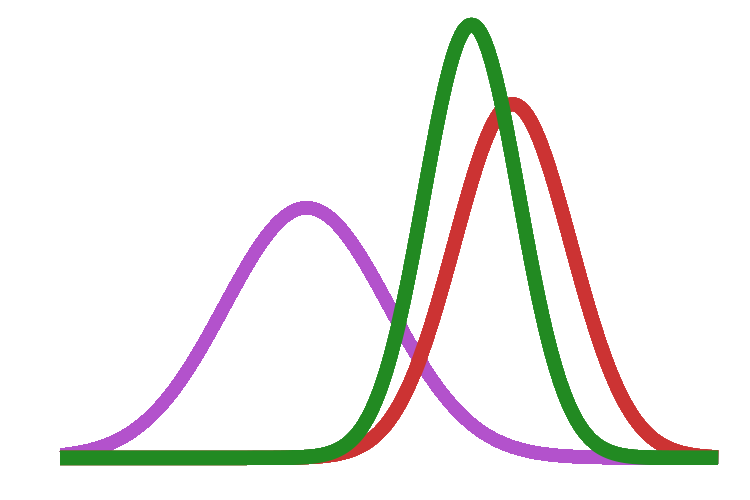
\includegraphics[width=0.9\textwidth]{turing.png}
		\end{column}
		\begin{column}{0.5\textwidth}
			\centering
			
\includegraphics[width=0.7\textwidth]{stan.png}
		\end{column}
	\end{columns}
\end{frame}

\begin{frame}{Why \texttt{Turing.jl}}
	\begin{vfilleditems}
		\item \textbf{Julia} all the way down...
		\item Can \textbf{interface/compose} with \textit{any} Julia package.
		\item Decoupling of \textbf{modeling DSL, inference algorithms and data}.
		\item Not only HMC-NUTS, but a whole \textbf{plethora of MCMC algorithms}, e.g. Metropolis-Hastings, Gibbs, SMC, IS etc.
		\item Easy to \textbf{create/prototype/modify inference algorithms}.
		\item \textbf{Transparent MCMC workflow}, e.g. iterative sampling API allows step-wise execution and debugging of the inference algorithm
		\item Very easy to \textbf{do stuff in the GPU}, e.g. NVIDIA's \texttt{CUDA.jl}, AMD's \texttt{AMDGPU.jl}, and Intel's \texttt{oneAPI.jl}.
		\item Very easy to do \textbf{distributed model inference and prediction}.
	\end{vfilleditems}
\end{frame}

\begin{frame}{Why \textit{not} \texttt{Turing}}
	\begin{vfilleditems}
	\item \textbf{Not as fast}, but pretty close behind, as \texttt{Stan}.
	\item \textbf{Not enough learning materials}, example models, tutorials.
	Also documentation is somewhat lacking in certain areas, e.g. \texttt{Bijectors.jl}.
	\item \textbf{Not as many citations as \texttt{Stan}},
	although not very far behind in GitHub stars.
	\item \textbf{Not well-known in the academic community}.
	\end{vfilleditems}
\end{frame}

\begin{frame}{Why \texttt{Stan}}
	\begin{vfilleditems}
	\item API for R, Python and Julia.
	\item Faster than \texttt{Turing.jl} in 95\% of models.
	\item \textbf{Well-known in the academic community}.
	\item \textbf{High citation count}.
	\item \textebf{More tutorials, example models, and learning materials available}.
	\end{vfilleditems}
\end{frame}

\begin{frame}{Why \textit{not} \texttt{Stan}}
	\begin{vfilleditems}
	\item If you want to try \textbf{something new}, you'll have to do in \textbf{C++}.
	\item Constrained \textbf{only to HMC-NUTS} as MCMC algorithm.
	\item \textbf{Cannot decouple model DSL from data} (and also from inference algorithm).
	\item \textbf{Does not compose well with other packages}.
	For anything you want to do, it has to ``exist'' in the \texttt{Stan} world,
	e.g. \texttt{bayesplot}.
	\item A \textbf{not so easy and intuitive ODE interface}.
	\item \textbf{GPU interface depends on OpenCL}.
	Also not easy to interoperate.
	\end{vfilleditems}
\end{frame}
